\documentclass[twoside]{book}

% Packages required by doxygen
\usepackage{fixltx2e}
\usepackage{calc}
\usepackage{doxygen}
\usepackage[export]{adjustbox} % also loads graphicx
\usepackage{graphicx}
\usepackage[utf8]{inputenc}
\usepackage{makeidx}
\usepackage{multicol}
\usepackage{multirow}
\PassOptionsToPackage{warn}{textcomp}
\usepackage{textcomp}
\usepackage[nointegrals]{wasysym}
\usepackage[table]{xcolor}

% Font selection
\usepackage[T1]{fontenc}
\usepackage[scaled=.90]{helvet}
\usepackage{courier}
\usepackage{amssymb}
\usepackage{sectsty}
\renewcommand{\familydefault}{\sfdefault}
\allsectionsfont{%
  \fontseries{bc}\selectfont%
  \color{darkgray}%
}
\renewcommand{\DoxyLabelFont}{%
  \fontseries{bc}\selectfont%
  \color{darkgray}%
}
\newcommand{\+}{\discretionary{\mbox{\scriptsize$\hookleftarrow$}}{}{}}

% Page & text layout
\usepackage{geometry}
\geometry{%
  a4paper,%
  top=2.5cm,%
  bottom=2.5cm,%
  left=2.5cm,%
  right=2.5cm%
}
\tolerance=750
\hfuzz=15pt
\hbadness=750
\setlength{\emergencystretch}{15pt}
\setlength{\parindent}{0cm}
\setlength{\parskip}{3ex plus 2ex minus 2ex}
\makeatletter
\renewcommand{\paragraph}{%
  \@startsection{paragraph}{4}{0ex}{-1.0ex}{1.0ex}{%
    \normalfont\normalsize\bfseries\SS@parafont%
  }%
}
\renewcommand{\subparagraph}{%
  \@startsection{subparagraph}{5}{0ex}{-1.0ex}{1.0ex}{%
    \normalfont\normalsize\bfseries\SS@subparafont%
  }%
}
\makeatother

% Headers & footers
\usepackage{fancyhdr}
\pagestyle{fancyplain}
\fancyhead[LE]{\fancyplain{}{\bfseries\thepage}}
\fancyhead[CE]{\fancyplain{}{}}
\fancyhead[RE]{\fancyplain{}{\bfseries\leftmark}}
\fancyhead[LO]{\fancyplain{}{\bfseries\rightmark}}
\fancyhead[CO]{\fancyplain{}{}}
\fancyhead[RO]{\fancyplain{}{\bfseries\thepage}}
\fancyfoot[LE]{\fancyplain{}{}}
\fancyfoot[CE]{\fancyplain{}{}}
\fancyfoot[RE]{\fancyplain{}{\bfseries\scriptsize Generated by Doxygen }}
\fancyfoot[LO]{\fancyplain{}{\bfseries\scriptsize Generated by Doxygen }}
\fancyfoot[CO]{\fancyplain{}{}}
\fancyfoot[RO]{\fancyplain{}{}}
\renewcommand{\footrulewidth}{0.4pt}
\renewcommand{\chaptermark}[1]{%
  \markboth{#1}{}%
}
\renewcommand{\sectionmark}[1]{%
  \markright{\thesection\ #1}%
}

% Indices & bibliography
\usepackage{natbib}
\usepackage[titles]{tocloft}
\setcounter{tocdepth}{3}
\setcounter{secnumdepth}{5}
\makeindex

% Hyperlinks (required, but should be loaded last)
\usepackage{ifpdf}
\ifpdf
  \usepackage[pdftex,pagebackref=true]{hyperref}
\else
  \usepackage[ps2pdf,pagebackref=true]{hyperref}
\fi
\hypersetup{%
  colorlinks=true,%
  linkcolor=blue,%
  citecolor=blue,%
  unicode%
}

% Custom commands
\newcommand{\clearemptydoublepage}{%
  \newpage{\pagestyle{empty}\cleardoublepage}%
}

\usepackage{caption}
\captionsetup{labelsep=space,justification=centering,font={bf},singlelinecheck=off,skip=4pt,position=top}

%===== C O N T E N T S =====

\begin{document}

% Titlepage & ToC
\hypersetup{pageanchor=false,
             bookmarksnumbered=true,
             pdfencoding=unicode
            }
\pagenumbering{alph}
\begin{titlepage}
\vspace*{7cm}
\begin{center}%
{\Large Gomoku \\[1ex]\large 024 }\\
\vspace*{1cm}
{\large Generated by Doxygen 1.8.13}\\
\end{center}
\end{titlepage}
\clearemptydoublepage
\pagenumbering{roman}
\tableofcontents
\clearemptydoublepage
\pagenumbering{arabic}
\hypersetup{pageanchor=true}

%--- Begin generated contents ---
\chapter{Deprecated List}
\label{deprecated}
\Hypertarget{deprecated}

\begin{DoxyRefList}
\item[\label{deprecated__deprecated000001}%
\Hypertarget{deprecated__deprecated000001}%
Member \hyperlink{classLogger_a69ca833f3e3643333d718f0cce464f9b}{Logger\+:\+:purge\+Move\+Log} ()]
\end{DoxyRefList}
\chapter{Hierarchical Index}
\section{Class Hierarchy}
This inheritance list is sorted roughly, but not completely, alphabetically\+:\begin{DoxyCompactList}
\item \contentsline{section}{Board}{\pageref{classBoard}}{}
\item \contentsline{section}{Drawer}{\pageref{classDrawer}}{}
\begin{DoxyCompactList}
\item \contentsline{section}{Drawer\+Alternative}{\pageref{classDrawerAlternative}}{}
\item \contentsline{section}{Drawer\+Classic}{\pageref{classDrawerClassic}}{}
\item \contentsline{section}{Drawer\+Mess}{\pageref{classDrawerMess}}{}
\end{DoxyCompactList}
\item \contentsline{section}{Game\+Loop}{\pageref{classGameLoop}}{}
\item \contentsline{section}{Gomoku}{\pageref{classGomoku}}{}
\item \contentsline{section}{Logger}{\pageref{classLogger}}{}
\item \contentsline{section}{Menu}{\pageref{classMenu}}{}
\begin{DoxyCompactList}
\item \contentsline{section}{Main\+Menu}{\pageref{classMainMenu}}{}
\end{DoxyCompactList}
\item \contentsline{section}{Ranking}{\pageref{classRanking}}{}
\end{DoxyCompactList}

\chapter{Class Index}
\section{Class List}
Here are the classes, structs, unions and interfaces with brief descriptions\+:\begin{DoxyCompactList}
\item\contentsline{section}{\hyperlink{classBoard}{Board} }{\pageref{classBoard}}{}
\item\contentsline{section}{\hyperlink{classDrawer}{Drawer} }{\pageref{classDrawer}}{}
\item\contentsline{section}{\hyperlink{classDrawerAlternative}{Drawer\+Alternative} }{\pageref{classDrawerAlternative}}{}
\item\contentsline{section}{\hyperlink{classDrawerClassic}{Drawer\+Classic} }{\pageref{classDrawerClassic}}{}
\item\contentsline{section}{\hyperlink{classDrawerMess}{Drawer\+Mess} }{\pageref{classDrawerMess}}{}
\item\contentsline{section}{\hyperlink{classGameLoop}{Game\+Loop} }{\pageref{classGameLoop}}{}
\item\contentsline{section}{\hyperlink{classGomoku}{Gomoku} }{\pageref{classGomoku}}{}
\item\contentsline{section}{\hyperlink{classLogger}{Logger} }{\pageref{classLogger}}{}
\item\contentsline{section}{\hyperlink{classMainMenu}{Main\+Menu} }{\pageref{classMainMenu}}{}
\item\contentsline{section}{\hyperlink{classMenu}{Menu} }{\pageref{classMenu}}{}
\item\contentsline{section}{\hyperlink{classRanking}{Ranking} }{\pageref{classRanking}}{}
\end{DoxyCompactList}

\chapter{Class Documentation}
\hypertarget{classBoard}{}\section{Board Class Reference}
\label{classBoard}\index{Board@{Board}}


{\ttfamily \#include $<$Board.\+h$>$}



Collaboration diagram for Board\+:
\nopagebreak
\begin{figure}[H]
\begin{center}
\leavevmode
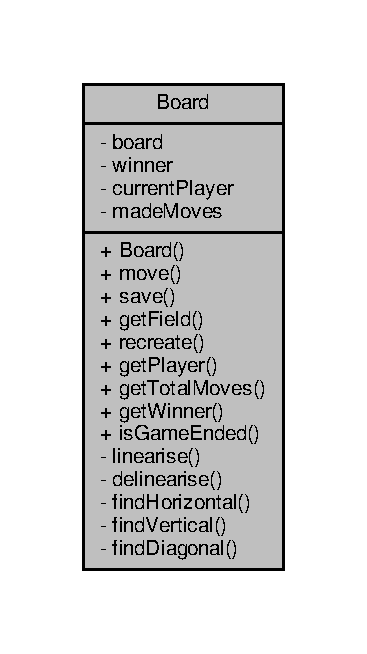
\includegraphics[width=176pt]{classBoard__coll__graph}
\end{center}
\end{figure}
\subsection*{Public Member Functions}
\begin{DoxyCompactItemize}
\item 
void \hyperlink{classBoard_a5ee56f4407f7792fe6f134a59d4af190}{move} (std\+::pair$<$ int, int $>$ position)
\item 
void \hyperlink{classBoard_afc8625b4719496080a988c294869d56a}{save} ()
\item 
int \hyperlink{classBoard_a2e57d7f5e62b0d870fb3ff1b76eb18ba}{get\+Field} (std\+::pair$<$ int, int $>$ position)
\item 
void \hyperlink{classBoard_aadae139aa7b1d53e7f9ae0ae0768f417}{recreate} ()
\item 
int \hyperlink{classBoard_ad4322f41e87c8a8a99e3424fb2a2a1ec}{get\+Player} ()
\item 
int \hyperlink{classBoard_aedc0672dfb6bddabc1c1cf091b483cbb}{get\+Total\+Moves} ()
\item 
int \hyperlink{classBoard_adef3bc4bb22a2f54b7703ceff15aea5b}{get\+Winner} ()
\item 
int \hyperlink{classBoard_afadc1ddff22c3a2ee25cad41ed7e5da0}{is\+Game\+Ended} ()
\end{DoxyCompactItemize}
\subsection*{Private Member Functions}
\begin{DoxyCompactItemize}
\item 
std\+::string \hyperlink{classBoard_a17ee7e0130537721b492cb7ed7235974}{linearise} ()
\item 
void \hyperlink{classBoard_a58de3d2bd69db7ef9258b3b907eb9de8}{delinearise} (std\+::string data)
\item 
int \hyperlink{classBoard_a2f984f83124db1b1df386ef9deff6a24}{find\+Horizontal} ()
\item 
int \hyperlink{classBoard_a4ee8b912055e8705e37a9b37125b70f0}{find\+Vertical} ()
\item 
int \hyperlink{classBoard_a99cff26f921e228dc11c381747381ced}{find\+Diagonal} ()
\end{DoxyCompactItemize}
\subsection*{Private Attributes}
\begin{DoxyCompactItemize}
\item 
int \hyperlink{classBoard_af588c465a63e9447a674398ec44446a9}{board} \mbox{[}15\mbox{]}\mbox{[}15\mbox{]}
\item 
int \hyperlink{classBoard_a67eeec840d17ab997e32234493ac7e39}{winner}
\item 
int \hyperlink{classBoard_a86b952cc745c2bd392f74434653457d3}{current\+Player}
\item 
int \hyperlink{classBoard_abfd418c2974974039da3fff24ad5c185}{made\+Moves}
\end{DoxyCompactItemize}


\subsection{Detailed Description}
Class represents board on which players are playing. It is 15x15 fields size. Each player puts its marks on board. \hyperlink{classBoard}{Board} does not have \hyperlink{classDrawer}{Drawer} service in-\/built. It\textquotesingle{}s implemented in \hyperlink{classDrawer}{Drawer} Class. 

Definition at line 16 of file Board.\+h.



\subsection{Member Function Documentation}
\mbox{\Hypertarget{classBoard_a58de3d2bd69db7ef9258b3b907eb9de8}\label{classBoard_a58de3d2bd69db7ef9258b3b907eb9de8}} 
\index{Board@{Board}!delinearise@{delinearise}}
\index{delinearise@{delinearise}!Board@{Board}}
\subsubsection{\texorpdfstring{delinearise()}{delinearise()}}
{\footnotesize\ttfamily void Board\+::delinearise (\begin{DoxyParamCaption}\item[{std\+::string}]{data }\end{DoxyParamCaption})\hspace{0.3cm}{\ttfamily [private]}}

Translate game state from string into 2D array -\/$>$ board 
\begin{DoxyParams}{Parameters}
{\em data} & string we like to translate \\
\hline
\end{DoxyParams}


Definition at line 69 of file Board.\+cpp.

\mbox{\Hypertarget{classBoard_a99cff26f921e228dc11c381747381ced}\label{classBoard_a99cff26f921e228dc11c381747381ced}} 
\index{Board@{Board}!find\+Diagonal@{find\+Diagonal}}
\index{find\+Diagonal@{find\+Diagonal}!Board@{Board}}
\subsubsection{\texorpdfstring{find\+Diagonal()}{findDiagonal()}}
{\footnotesize\ttfamily int Board\+::find\+Diagonal (\begin{DoxyParamCaption}{ }\end{DoxyParamCaption})\hspace{0.3cm}{\ttfamily [private]}}

Same as previous, but performed in diagonals \begin{DoxyReturn}{Returns}
player number if any player won, or 0 if not 
\end{DoxyReturn}


Definition at line 133 of file Board.\+cpp.

\mbox{\Hypertarget{classBoard_a2f984f83124db1b1df386ef9deff6a24}\label{classBoard_a2f984f83124db1b1df386ef9deff6a24}} 
\index{Board@{Board}!find\+Horizontal@{find\+Horizontal}}
\index{find\+Horizontal@{find\+Horizontal}!Board@{Board}}
\subsubsection{\texorpdfstring{find\+Horizontal()}{findHorizontal()}}
{\footnotesize\ttfamily int Board\+::find\+Horizontal (\begin{DoxyParamCaption}{ }\end{DoxyParamCaption})\hspace{0.3cm}{\ttfamily [private]}}

Check if in any row was 5 the same signs \begin{DoxyReturn}{Returns}
player number if any player won, or 0 if not 
\end{DoxyReturn}


Definition at line 106 of file Board.\+cpp.

\mbox{\Hypertarget{classBoard_a4ee8b912055e8705e37a9b37125b70f0}\label{classBoard_a4ee8b912055e8705e37a9b37125b70f0}} 
\index{Board@{Board}!find\+Vertical@{find\+Vertical}}
\index{find\+Vertical@{find\+Vertical}!Board@{Board}}
\subsubsection{\texorpdfstring{find\+Vertical()}{findVertical()}}
{\footnotesize\ttfamily int Board\+::find\+Vertical (\begin{DoxyParamCaption}{ }\end{DoxyParamCaption})\hspace{0.3cm}{\ttfamily [private]}}

Same as previous but performed in columns \begin{DoxyReturn}{Returns}
player number if any player won, or 0 if not 
\end{DoxyReturn}


Definition at line 119 of file Board.\+cpp.

\mbox{\Hypertarget{classBoard_a2e57d7f5e62b0d870fb3ff1b76eb18ba}\label{classBoard_a2e57d7f5e62b0d870fb3ff1b76eb18ba}} 
\index{Board@{Board}!get\+Field@{get\+Field}}
\index{get\+Field@{get\+Field}!Board@{Board}}
\subsubsection{\texorpdfstring{get\+Field()}{getField()}}
{\footnotesize\ttfamily int Board\+::get\+Field (\begin{DoxyParamCaption}\item[{std\+::pair$<$ int, int $>$}]{position }\end{DoxyParamCaption})}

Returns mark on pointed field 
\begin{DoxyParams}{Parameters}
{\em position} & position wich we\textquotesingle{}d like to check \\
\hline
\end{DoxyParams}
\begin{DoxyReturn}{Returns}
mark as number 
\end{DoxyReturn}


Definition at line 52 of file Board.\+cpp.

\mbox{\Hypertarget{classBoard_ad4322f41e87c8a8a99e3424fb2a2a1ec}\label{classBoard_ad4322f41e87c8a8a99e3424fb2a2a1ec}} 
\index{Board@{Board}!get\+Player@{get\+Player}}
\index{get\+Player@{get\+Player}!Board@{Board}}
\subsubsection{\texorpdfstring{get\+Player()}{getPlayer()}}
{\footnotesize\ttfamily int Board\+::get\+Player (\begin{DoxyParamCaption}{ }\end{DoxyParamCaption})}

Getter for current player \begin{DoxyReturn}{Returns}
current player as number 
\end{DoxyReturn}


Definition at line 77 of file Board.\+cpp.

\mbox{\Hypertarget{classBoard_aedc0672dfb6bddabc1c1cf091b483cbb}\label{classBoard_aedc0672dfb6bddabc1c1cf091b483cbb}} 
\index{Board@{Board}!get\+Total\+Moves@{get\+Total\+Moves}}
\index{get\+Total\+Moves@{get\+Total\+Moves}!Board@{Board}}
\subsubsection{\texorpdfstring{get\+Total\+Moves()}{getTotalMoves()}}
{\footnotesize\ttfamily int Board\+::get\+Total\+Moves (\begin{DoxyParamCaption}{ }\end{DoxyParamCaption})}

Getter for total number of made moves during this game \begin{DoxyReturn}{Returns}
total number of moves 
\end{DoxyReturn}


Definition at line 81 of file Board.\+cpp.

\mbox{\Hypertarget{classBoard_adef3bc4bb22a2f54b7703ceff15aea5b}\label{classBoard_adef3bc4bb22a2f54b7703ceff15aea5b}} 
\index{Board@{Board}!get\+Winner@{get\+Winner}}
\index{get\+Winner@{get\+Winner}!Board@{Board}}
\subsubsection{\texorpdfstring{get\+Winner()}{getWinner()}}
{\footnotesize\ttfamily int Board\+::get\+Winner (\begin{DoxyParamCaption}{ }\end{DoxyParamCaption})}

Getter for winner player \begin{DoxyReturn}{Returns}
winner player 
\end{DoxyReturn}


Definition at line 164 of file Board.\+cpp.

\mbox{\Hypertarget{classBoard_afadc1ddff22c3a2ee25cad41ed7e5da0}\label{classBoard_afadc1ddff22c3a2ee25cad41ed7e5da0}} 
\index{Board@{Board}!is\+Game\+Ended@{is\+Game\+Ended}}
\index{is\+Game\+Ended@{is\+Game\+Ended}!Board@{Board}}
\subsubsection{\texorpdfstring{is\+Game\+Ended()}{isGameEnded()}}
{\footnotesize\ttfamily int Board\+::is\+Game\+Ended (\begin{DoxyParamCaption}{ }\end{DoxyParamCaption})}

Check if endgame condition is fulfiled \begin{DoxyReturn}{Returns}
player number if any player won, or 0 if not 
\end{DoxyReturn}


Definition at line 85 of file Board.\+cpp.

\mbox{\Hypertarget{classBoard_a17ee7e0130537721b492cb7ed7235974}\label{classBoard_a17ee7e0130537721b492cb7ed7235974}} 
\index{Board@{Board}!linearise@{linearise}}
\index{linearise@{linearise}!Board@{Board}}
\subsubsection{\texorpdfstring{linearise()}{linearise()}}
{\footnotesize\ttfamily std\+::string Board\+::linearise (\begin{DoxyParamCaption}{ }\end{DoxyParamCaption})\hspace{0.3cm}{\ttfamily [private]}}

Function linearise bord into string, which is used to save game progress \begin{DoxyReturn}{Returns}
board as linearised string 
\end{DoxyReturn}


Definition at line 10 of file Board.\+cpp.

\mbox{\Hypertarget{classBoard_a5ee56f4407f7792fe6f134a59d4af190}\label{classBoard_a5ee56f4407f7792fe6f134a59d4af190}} 
\index{Board@{Board}!move@{move}}
\index{move@{move}!Board@{Board}}
\subsubsection{\texorpdfstring{move()}{move()}}
{\footnotesize\ttfamily void Board\+::move (\begin{DoxyParamCaption}\item[{std\+::pair$<$ int, int $>$}]{position }\end{DoxyParamCaption})}

Update board with player move. Notice players are choosen by function no by caller. 
\begin{DoxyParams}{Parameters}
{\em position} & position on which we put mark \\
\hline
\end{DoxyParams}


Definition at line 32 of file Board.\+cpp.

\mbox{\Hypertarget{classBoard_aadae139aa7b1d53e7f9ae0ae0768f417}\label{classBoard_aadae139aa7b1d53e7f9ae0ae0768f417}} 
\index{Board@{Board}!recreate@{recreate}}
\index{recreate@{recreate}!Board@{Board}}
\subsubsection{\texorpdfstring{recreate()}{recreate()}}
{\footnotesize\ttfamily void Board\+::recreate (\begin{DoxyParamCaption}{ }\end{DoxyParamCaption})}

Recreates board state after save 

Definition at line 58 of file Board.\+cpp.

\mbox{\Hypertarget{classBoard_afc8625b4719496080a988c294869d56a}\label{classBoard_afc8625b4719496080a988c294869d56a}} 
\index{Board@{Board}!save@{save}}
\index{save@{save}!Board@{Board}}
\subsubsection{\texorpdfstring{save()}{save()}}
{\footnotesize\ttfamily void Board\+::save (\begin{DoxyParamCaption}{ }\end{DoxyParamCaption})}

Save game state to file -\/$>$ Game.\+save 

Definition at line 43 of file Board.\+cpp.



\subsection{Member Data Documentation}
\mbox{\Hypertarget{classBoard_af588c465a63e9447a674398ec44446a9}\label{classBoard_af588c465a63e9447a674398ec44446a9}} 
\index{Board@{Board}!board@{board}}
\index{board@{board}!Board@{Board}}
\subsubsection{\texorpdfstring{board}{board}}
{\footnotesize\ttfamily int Board\+::board\mbox{[}15\mbox{]}\mbox{[}15\mbox{]}\hspace{0.3cm}{\ttfamily [private]}}

Actual board 

Definition at line 21 of file Board.\+h.

\mbox{\Hypertarget{classBoard_a86b952cc745c2bd392f74434653457d3}\label{classBoard_a86b952cc745c2bd392f74434653457d3}} 
\index{Board@{Board}!current\+Player@{current\+Player}}
\index{current\+Player@{current\+Player}!Board@{Board}}
\subsubsection{\texorpdfstring{current\+Player}{currentPlayer}}
{\footnotesize\ttfamily int Board\+::current\+Player\hspace{0.3cm}{\ttfamily [private]}}

Number of player which made move. Updated after move was made 

Definition at line 44 of file Board.\+h.

\mbox{\Hypertarget{classBoard_abfd418c2974974039da3fff24ad5c185}\label{classBoard_abfd418c2974974039da3fff24ad5c185}} 
\index{Board@{Board}!made\+Moves@{made\+Moves}}
\index{made\+Moves@{made\+Moves}!Board@{Board}}
\subsubsection{\texorpdfstring{made\+Moves}{madeMoves}}
{\footnotesize\ttfamily int Board\+::made\+Moves\hspace{0.3cm}{\ttfamily [private]}}

Number of made moves. Updated after move was made 

Definition at line 50 of file Board.\+h.

\mbox{\Hypertarget{classBoard_a67eeec840d17ab997e32234493ac7e39}\label{classBoard_a67eeec840d17ab997e32234493ac7e39}} 
\index{Board@{Board}!winner@{winner}}
\index{winner@{winner}!Board@{Board}}
\subsubsection{\texorpdfstring{winner}{winner}}
{\footnotesize\ttfamily int Board\+::winner\hspace{0.3cm}{\ttfamily [private]}}

Player which won 

Definition at line 26 of file Board.\+h.



The documentation for this class was generated from the following files\+:\begin{DoxyCompactItemize}
\item 
headers/Board.\+h\item 
classes/Board.\+cpp\end{DoxyCompactItemize}

\hypertarget{classDrawer}{}\section{Drawer Class Reference}
\label{classDrawer}\index{Drawer@{Drawer}}


{\ttfamily \#include $<$Drawer.\+h$>$}



Inheritance diagram for Drawer\+:
\nopagebreak
\begin{figure}[H]
\begin{center}
\leavevmode
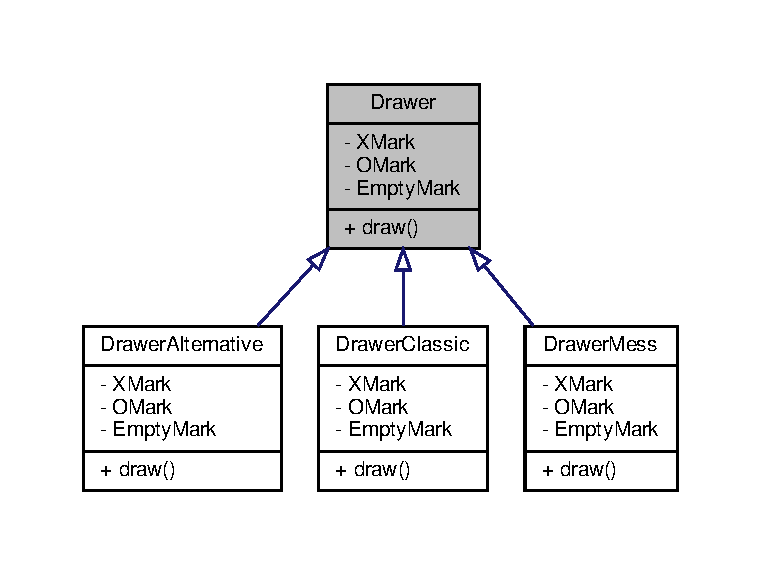
\includegraphics[width=350pt]{classDrawer__inherit__graph}
\end{center}
\end{figure}


Collaboration diagram for Drawer\+:
\nopagebreak
\begin{figure}[H]
\begin{center}
\leavevmode
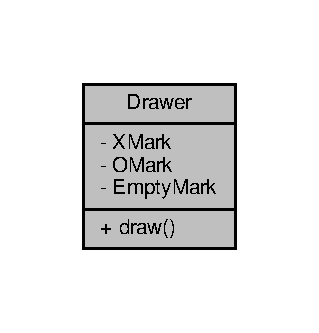
\includegraphics[width=153pt]{classDrawer__coll__graph}
\end{center}
\end{figure}
\subsection*{Public Member Functions}
\begin{DoxyCompactItemize}
\item 
virtual void \hyperlink{classDrawer_afe75fce45596f02f01514322ebd57c8c}{draw} (\hyperlink{classBoard}{Board} board)=0
\end{DoxyCompactItemize}
\subsection*{Private Attributes}
\begin{DoxyCompactItemize}
\item 
\mbox{\Hypertarget{classDrawer_a86db125a08ba0e79d545542a69fde9d3}\label{classDrawer_a86db125a08ba0e79d545542a69fde9d3}} 
const std\+::string {\bfseries X\+Mark}
\item 
\mbox{\Hypertarget{classDrawer_a007403c532527c21334e81e214109676}\label{classDrawer_a007403c532527c21334e81e214109676}} 
const std\+::string {\bfseries O\+Mark}
\item 
\mbox{\Hypertarget{classDrawer_a673b951b13d86a6d46bde89029f149b3}\label{classDrawer_a673b951b13d86a6d46bde89029f149b3}} 
const std\+::string {\bfseries Empty\+Mark}
\end{DoxyCompactItemize}


\subsection{Detailed Description}
\hyperlink{classDrawer}{Drawer} class represents in console current \hyperlink{classBoard}{Board} state. \hyperlink{classDrawer}{Drawer} is an abstract class which is implemented in its subclass \begin{DoxySeeAlso}{See also}
\hyperlink{classDrawerClassic}{Drawer\+Classic} 

\hyperlink{classDrawerAlternative}{Drawer\+Alternative} 

\hyperlink{classDrawerMess}{Drawer\+Mess} 
\end{DoxySeeAlso}


Definition at line 19 of file Drawer.\+h.



\subsection{Member Function Documentation}
\mbox{\Hypertarget{classDrawer_afe75fce45596f02f01514322ebd57c8c}\label{classDrawer_afe75fce45596f02f01514322ebd57c8c}} 
\index{Drawer@{Drawer}!draw@{draw}}
\index{draw@{draw}!Drawer@{Drawer}}
\subsubsection{\texorpdfstring{draw()}{draw()}}
{\footnotesize\ttfamily virtual void Drawer\+::draw (\begin{DoxyParamCaption}\item[{\hyperlink{classBoard}{Board}}]{board }\end{DoxyParamCaption})\hspace{0.3cm}{\ttfamily [pure virtual]}}

Draws \hyperlink{classBoard}{Board} on screen 
\begin{DoxyParams}{Parameters}
{\em board} & board which should be drawn \\
\hline
\end{DoxyParams}


Implemented in \hyperlink{classDrawerMess_a6d682acdf4ad01f370f9985cacd606a9}{Drawer\+Mess}, \hyperlink{classDrawerAlternative_a2d56b61df9a3878c9aa24db5896578ba}{Drawer\+Alternative}, and \hyperlink{classDrawerClassic_ab5e18d90571afab9a2b8482b2d9d8264}{Drawer\+Classic}.



The documentation for this class was generated from the following file\+:\begin{DoxyCompactItemize}
\item 
headers/Drawer.\+h\end{DoxyCompactItemize}

\hypertarget{classDrawerAlternative}{}\section{Drawer\+Alternative Class Reference}
\label{classDrawerAlternative}\index{Drawer\+Alternative@{Drawer\+Alternative}}


{\ttfamily \#include $<$Drawer\+Alternative.\+h$>$}



Inheritance diagram for Drawer\+Alternative\+:
\nopagebreak
\begin{figure}[H]
\begin{center}
\leavevmode
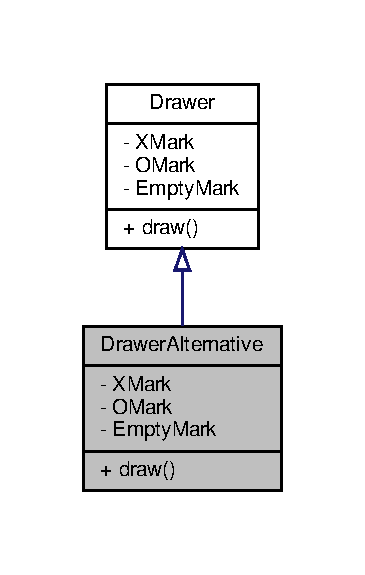
\includegraphics[width=175pt]{classDrawerAlternative__inherit__graph}
\end{center}
\end{figure}


Collaboration diagram for Drawer\+Alternative\+:
\nopagebreak
\begin{figure}[H]
\begin{center}
\leavevmode
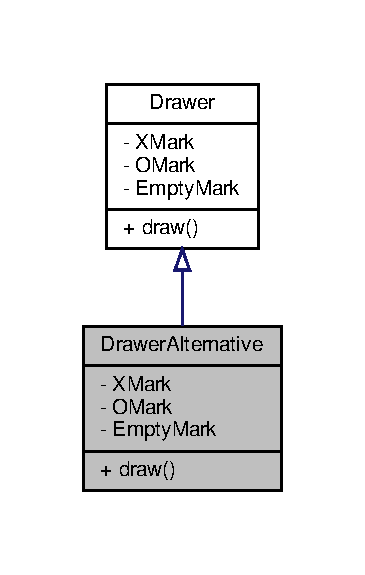
\includegraphics[width=175pt]{classDrawerAlternative__coll__graph}
\end{center}
\end{figure}
\subsection*{Public Member Functions}
\begin{DoxyCompactItemize}
\item 
virtual void \hyperlink{classDrawerAlternative_a2d56b61df9a3878c9aa24db5896578ba}{draw} (\hyperlink{classBoard}{Board} board) override
\end{DoxyCompactItemize}
\subsection*{Private Attributes}
\begin{DoxyCompactItemize}
\item 
\mbox{\Hypertarget{classDrawerAlternative_a58688e22709b37e5fdcf4ce5d5a73b96}\label{classDrawerAlternative_a58688e22709b37e5fdcf4ce5d5a73b96}} 
const std\+::string {\bfseries X\+Mark} = \char`\"{}+\char`\"{}
\item 
\mbox{\Hypertarget{classDrawerAlternative_a4f80da586b01bab01119d2a76fe39a95}\label{classDrawerAlternative_a4f80da586b01bab01119d2a76fe39a95}} 
const std\+::string {\bfseries O\+Mark} = \char`\"{}o\char`\"{}
\item 
\mbox{\Hypertarget{classDrawerAlternative_a11d00e3321f98034af61d70f570b19aa}\label{classDrawerAlternative_a11d00e3321f98034af61d70f570b19aa}} 
const std\+::string {\bfseries Empty\+Mark} = \char`\"{} \char`\"{}
\end{DoxyCompactItemize}


\subsection{Detailed Description}
Is implementation of \hyperlink{classDrawer}{Drawer}. In this version player1 is + and player2 is o. 

Definition at line 16 of file Drawer\+Alternative.\+h.



\subsection{Member Function Documentation}
\mbox{\Hypertarget{classDrawerAlternative_a2d56b61df9a3878c9aa24db5896578ba}\label{classDrawerAlternative_a2d56b61df9a3878c9aa24db5896578ba}} 
\index{Drawer\+Alternative@{Drawer\+Alternative}!draw@{draw}}
\index{draw@{draw}!Drawer\+Alternative@{Drawer\+Alternative}}
\subsubsection{\texorpdfstring{draw()}{draw()}}
{\footnotesize\ttfamily void Drawer\+Alternative\+::draw (\begin{DoxyParamCaption}\item[{\hyperlink{classBoard}{Board}}]{board }\end{DoxyParamCaption})\hspace{0.3cm}{\ttfamily [override]}, {\ttfamily [virtual]}}

Draws \hyperlink{classBoard}{Board} on screen 
\begin{DoxyParams}{Parameters}
{\em board} & board which should be drawn \\
\hline
\end{DoxyParams}


Implements \hyperlink{classDrawer_afe75fce45596f02f01514322ebd57c8c}{Drawer}.



Definition at line 8 of file Drawer\+Alternative.\+cpp.



The documentation for this class was generated from the following files\+:\begin{DoxyCompactItemize}
\item 
headers/Drawer\+Alternative.\+h\item 
classes/Drawer\+Alternative.\+cpp\end{DoxyCompactItemize}

\hypertarget{classDrawerClassic}{}\section{Drawer\+Classic Class Reference}
\label{classDrawerClassic}\index{Drawer\+Classic@{Drawer\+Classic}}


{\ttfamily \#include $<$Drawer\+Classic.\+h$>$}



Inheritance diagram for Drawer\+Classic\+:
\nopagebreak
\begin{figure}[H]
\begin{center}
\leavevmode
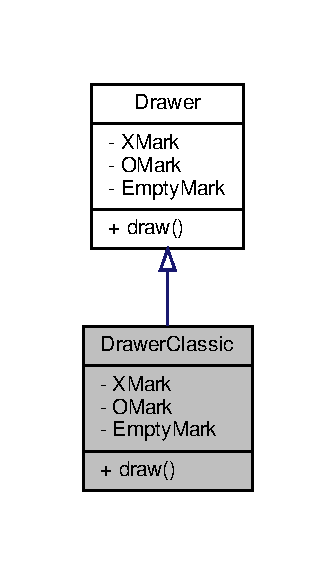
\includegraphics[width=161pt]{classDrawerClassic__inherit__graph}
\end{center}
\end{figure}


Collaboration diagram for Drawer\+Classic\+:
\nopagebreak
\begin{figure}[H]
\begin{center}
\leavevmode
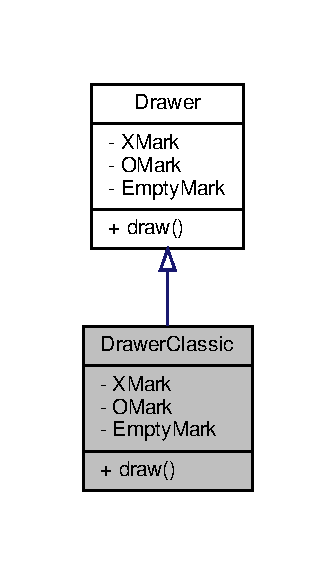
\includegraphics[width=161pt]{classDrawerClassic__coll__graph}
\end{center}
\end{figure}
\subsection*{Public Member Functions}
\begin{DoxyCompactItemize}
\item 
virtual void \hyperlink{classDrawerClassic_ab5e18d90571afab9a2b8482b2d9d8264}{draw} (\hyperlink{classBoard}{Board} board) override
\end{DoxyCompactItemize}
\subsection*{Private Attributes}
\begin{DoxyCompactItemize}
\item 
\mbox{\Hypertarget{classDrawerClassic_a31aba72f2a6463a1ad4a6974c31b65ae}\label{classDrawerClassic_a31aba72f2a6463a1ad4a6974c31b65ae}} 
const std\+::string {\bfseries X\+Mark} = \char`\"{}X\char`\"{}
\item 
\mbox{\Hypertarget{classDrawerClassic_a5f1c89c7c6d37eb435f447f1a5934e2b}\label{classDrawerClassic_a5f1c89c7c6d37eb435f447f1a5934e2b}} 
const std\+::string {\bfseries O\+Mark} = \char`\"{}O\char`\"{}
\item 
\mbox{\Hypertarget{classDrawerClassic_a9d79d07a7b0d24a5c8cd3bbfb4e60d44}\label{classDrawerClassic_a9d79d07a7b0d24a5c8cd3bbfb4e60d44}} 
const std\+::string {\bfseries Empty\+Mark} = \char`\"{} \char`\"{}
\end{DoxyCompactItemize}


\subsection{Detailed Description}
Is implementation of \hyperlink{classDrawer}{Drawer}. In this version player1 is X and player2 is O. 

Definition at line 15 of file Drawer\+Classic.\+h.



\subsection{Member Function Documentation}
\mbox{\Hypertarget{classDrawerClassic_ab5e18d90571afab9a2b8482b2d9d8264}\label{classDrawerClassic_ab5e18d90571afab9a2b8482b2d9d8264}} 
\index{Drawer\+Classic@{Drawer\+Classic}!draw@{draw}}
\index{draw@{draw}!Drawer\+Classic@{Drawer\+Classic}}
\subsubsection{\texorpdfstring{draw()}{draw()}}
{\footnotesize\ttfamily void Drawer\+Classic\+::draw (\begin{DoxyParamCaption}\item[{\hyperlink{classBoard}{Board}}]{board }\end{DoxyParamCaption})\hspace{0.3cm}{\ttfamily [override]}, {\ttfamily [virtual]}}

Draws \hyperlink{classBoard}{Board} on screen 
\begin{DoxyParams}{Parameters}
{\em board} & board which should be drawn \\
\hline
\end{DoxyParams}


Implements \hyperlink{classDrawer_afe75fce45596f02f01514322ebd57c8c}{Drawer}.



Definition at line 8 of file Drawer\+Classic.\+cpp.



The documentation for this class was generated from the following files\+:\begin{DoxyCompactItemize}
\item 
headers/Drawer\+Classic.\+h\item 
classes/Drawer\+Classic.\+cpp\end{DoxyCompactItemize}

\hypertarget{classDrawerMess}{}\section{Drawer\+Mess Class Reference}
\label{classDrawerMess}\index{Drawer\+Mess@{Drawer\+Mess}}


{\ttfamily \#include $<$Drawer\+Mess.\+h$>$}



Inheritance diagram for Drawer\+Mess\+:
\nopagebreak
\begin{figure}[H]
\begin{center}
\leavevmode
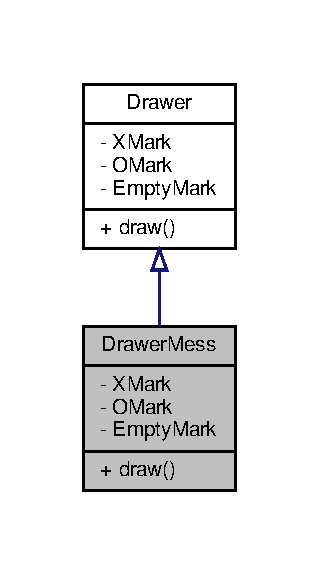
\includegraphics[width=153pt]{classDrawerMess__inherit__graph}
\end{center}
\end{figure}


Collaboration diagram for Drawer\+Mess\+:
\nopagebreak
\begin{figure}[H]
\begin{center}
\leavevmode
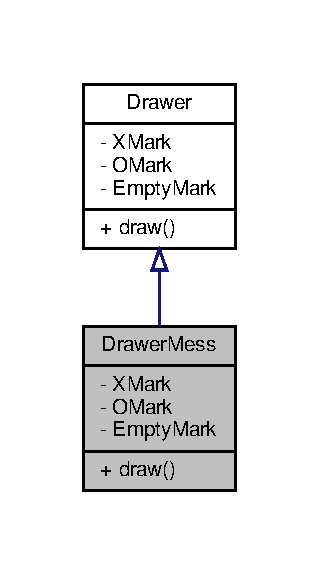
\includegraphics[width=153pt]{classDrawerMess__coll__graph}
\end{center}
\end{figure}
\subsection*{Public Member Functions}
\begin{DoxyCompactItemize}
\item 
virtual void \hyperlink{classDrawerMess_a6d682acdf4ad01f370f9985cacd606a9}{draw} (\hyperlink{classBoard}{Board} board) override
\end{DoxyCompactItemize}
\subsection*{Private Attributes}
\begin{DoxyCompactItemize}
\item 
\mbox{\Hypertarget{classDrawerMess_ab431d116153398b05905cffe8505544e}\label{classDrawerMess_ab431d116153398b05905cffe8505544e}} 
const std\+::string {\bfseries X\+Mark} = \char`\"{}X\char`\"{}
\item 
\mbox{\Hypertarget{classDrawerMess_aeafb5b339bba9f4ee02bf85f0126f05d}\label{classDrawerMess_aeafb5b339bba9f4ee02bf85f0126f05d}} 
const std\+::string {\bfseries O\+Mark} = \char`\"{}O\char`\"{}
\item 
\mbox{\Hypertarget{classDrawerMess_a315afa5f3ef89dcdec37bb876ead17ee}\label{classDrawerMess_a315afa5f3ef89dcdec37bb876ead17ee}} 
const std\+::string {\bfseries Empty\+Mark} = \char`\"{}.\char`\"{}
\end{DoxyCompactItemize}


\subsection{Detailed Description}
Is implementation of \hyperlink{classDrawer}{Drawer}. In this version player1 is X and player2 is O and empty fields are marked as dots. 

Definition at line 17 of file Drawer\+Mess.\+h.



\subsection{Member Function Documentation}
\mbox{\Hypertarget{classDrawerMess_a6d682acdf4ad01f370f9985cacd606a9}\label{classDrawerMess_a6d682acdf4ad01f370f9985cacd606a9}} 
\index{Drawer\+Mess@{Drawer\+Mess}!draw@{draw}}
\index{draw@{draw}!Drawer\+Mess@{Drawer\+Mess}}
\subsubsection{\texorpdfstring{draw()}{draw()}}
{\footnotesize\ttfamily void Drawer\+Mess\+::draw (\begin{DoxyParamCaption}\item[{\hyperlink{classBoard}{Board}}]{board }\end{DoxyParamCaption})\hspace{0.3cm}{\ttfamily [override]}, {\ttfamily [virtual]}}

Draws \hyperlink{classBoard}{Board} on screen 
\begin{DoxyParams}{Parameters}
{\em board} & board which should be drawn \\
\hline
\end{DoxyParams}


Implements \hyperlink{classDrawer_afe75fce45596f02f01514322ebd57c8c}{Drawer}.



Definition at line 13 of file Drawer\+Mess.\+cpp.



The documentation for this class was generated from the following files\+:\begin{DoxyCompactItemize}
\item 
headers/Drawer\+Mess.\+h\item 
classes/Drawer\+Mess.\+cpp\end{DoxyCompactItemize}

\hypertarget{classGameLoop}{}\section{Game\+Loop Class Reference}
\label{classGameLoop}\index{Game\+Loop@{Game\+Loop}}


{\ttfamily \#include $<$Game\+Loop.\+h$>$}



Collaboration diagram for Game\+Loop\+:
\nopagebreak
\begin{figure}[H]
\begin{center}
\leavevmode
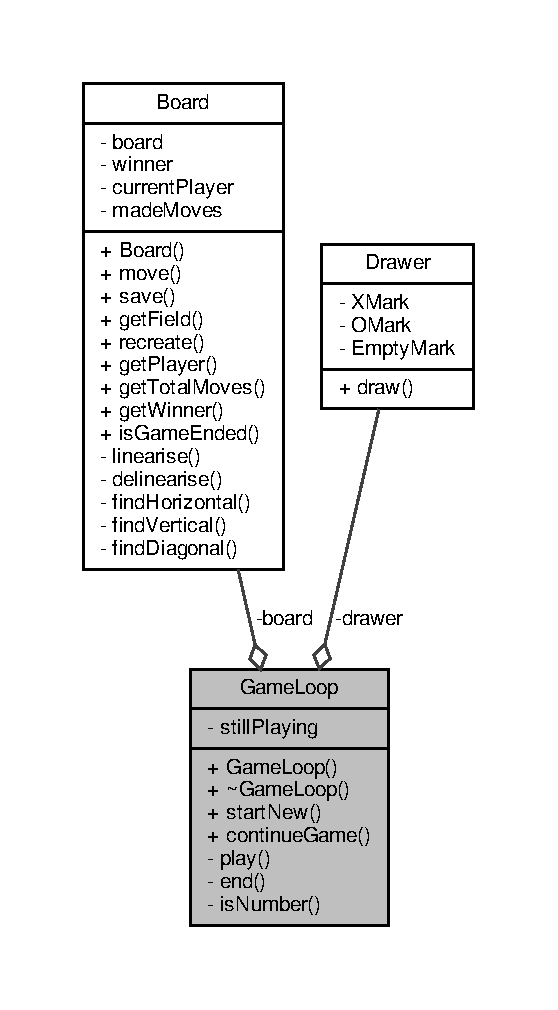
\includegraphics[width=268pt]{classGameLoop__coll__graph}
\end{center}
\end{figure}
\subsection*{Public Member Functions}
\begin{DoxyCompactItemize}
\item 
void \hyperlink{classGameLoop_a12718de4b3e9535288cc77c8d5f27979}{start\+New} ()
\item 
void \hyperlink{classGameLoop_adc88e75cb8106655d88296cc082767bc}{continue\+Game} ()
\end{DoxyCompactItemize}
\subsection*{Private Member Functions}
\begin{DoxyCompactItemize}
\item 
void \hyperlink{classGameLoop_a7e143e66d9a047a15d20c20da85f23d0}{play} ()
\item 
void \hyperlink{classGameLoop_a30733a30b29bc93c3009b62bde59ddde}{end} ()
\item 
void \hyperlink{classGameLoop_aef095ed6895919ae55e260b0149ff29a}{is\+Number} (std\+::string text)
\end{DoxyCompactItemize}
\subsection*{Private Attributes}
\begin{DoxyCompactItemize}
\item 
bool \hyperlink{classGameLoop_a74bff510eaf3cab91599f164dfa903cf}{still\+Playing}
\item 
\hyperlink{classBoard}{Board} \hyperlink{classGameLoop_a73ffb8954f2f2fd298e2bfe22be73ce6}{board}
\item 
\hyperlink{classDrawer}{Drawer} $\ast$ \hyperlink{classGameLoop_a9f25ffc0e91f10c6030ca6b05032f71f}{drawer}
\end{DoxyCompactItemize}


\subsection{Detailed Description}
Class which is main Game loop. Contains method for controlling game state. Class is not main Program loop, which is \hyperlink{classGomoku}{Gomoku} class 

Definition at line 17 of file Game\+Loop.\+h.



\subsection{Member Function Documentation}
\mbox{\Hypertarget{classGameLoop_adc88e75cb8106655d88296cc082767bc}\label{classGameLoop_adc88e75cb8106655d88296cc082767bc}} 
\index{Game\+Loop@{Game\+Loop}!continue\+Game@{continue\+Game}}
\index{continue\+Game@{continue\+Game}!Game\+Loop@{Game\+Loop}}
\subsubsection{\texorpdfstring{continue\+Game()}{continueGame()}}
{\footnotesize\ttfamily void Game\+Loop\+::continue\+Game (\begin{DoxyParamCaption}{ }\end{DoxyParamCaption})}

Loads last saved \hyperlink{classBoard}{Board} setup, and calls \hyperlink{classGameLoop_a7e143e66d9a047a15d20c20da85f23d0}{play()} 

Definition at line 24 of file Game\+Loop.\+cpp.

\mbox{\Hypertarget{classGameLoop_a30733a30b29bc93c3009b62bde59ddde}\label{classGameLoop_a30733a30b29bc93c3009b62bde59ddde}} 
\index{Game\+Loop@{Game\+Loop}!end@{end}}
\index{end@{end}!Game\+Loop@{Game\+Loop}}
\subsubsection{\texorpdfstring{end()}{end()}}
{\footnotesize\ttfamily void Game\+Loop\+::end (\begin{DoxyParamCaption}{ }\end{DoxyParamCaption})\hspace{0.3cm}{\ttfamily [private]}}

Called if game was won by one of the players. Notify who is the winner save results to \hyperlink{classRanking}{Ranking}, and save empty board, so choosing to continue in main menu don\textquotesingle{}t bring board with immediately winning setup 

Definition at line 89 of file Game\+Loop.\+cpp.

\mbox{\Hypertarget{classGameLoop_aef095ed6895919ae55e260b0149ff29a}\label{classGameLoop_aef095ed6895919ae55e260b0149ff29a}} 
\index{Game\+Loop@{Game\+Loop}!is\+Number@{is\+Number}}
\index{is\+Number@{is\+Number}!Game\+Loop@{Game\+Loop}}
\subsubsection{\texorpdfstring{is\+Number()}{isNumber()}}
{\footnotesize\ttfamily void Game\+Loop\+::is\+Number (\begin{DoxyParamCaption}\item[{std\+::string}]{text }\end{DoxyParamCaption})\hspace{0.3cm}{\ttfamily [private]}}

Check if given text is a unsigned int 
\begin{DoxyParams}{Parameters}
{\em text} & value to check \\
\hline
\end{DoxyParams}


Definition at line 78 of file Game\+Loop.\+cpp.

\mbox{\Hypertarget{classGameLoop_a7e143e66d9a047a15d20c20da85f23d0}\label{classGameLoop_a7e143e66d9a047a15d20c20da85f23d0}} 
\index{Game\+Loop@{Game\+Loop}!play@{play}}
\index{play@{play}!Game\+Loop@{Game\+Loop}}
\subsubsection{\texorpdfstring{play()}{play()}}
{\footnotesize\ttfamily void Game\+Loop\+::play (\begin{DoxyParamCaption}{ }\end{DoxyParamCaption})\hspace{0.3cm}{\ttfamily [private]}}

Function which reads user inputs, and calls \hyperlink{classBoard}{Board} and \hyperlink{classDrawer}{Drawer}, as well as checking if inputs was valid, and if player wants to exit game 

Definition at line 30 of file Game\+Loop.\+cpp.

\mbox{\Hypertarget{classGameLoop_a12718de4b3e9535288cc77c8d5f27979}\label{classGameLoop_a12718de4b3e9535288cc77c8d5f27979}} 
\index{Game\+Loop@{Game\+Loop}!start\+New@{start\+New}}
\index{start\+New@{start\+New}!Game\+Loop@{Game\+Loop}}
\subsubsection{\texorpdfstring{start\+New()}{startNew()}}
{\footnotesize\ttfamily void Game\+Loop\+::start\+New (\begin{DoxyParamCaption}{ }\end{DoxyParamCaption})}

Starts new game, just calls \hyperlink{classGameLoop_a7e143e66d9a047a15d20c20da85f23d0}{play()} function 

Definition at line 20 of file Game\+Loop.\+cpp.



\subsection{Member Data Documentation}
\mbox{\Hypertarget{classGameLoop_a73ffb8954f2f2fd298e2bfe22be73ce6}\label{classGameLoop_a73ffb8954f2f2fd298e2bfe22be73ce6}} 
\index{Game\+Loop@{Game\+Loop}!board@{board}}
\index{board@{board}!Game\+Loop@{Game\+Loop}}
\subsubsection{\texorpdfstring{board}{board}}
{\footnotesize\ttfamily \hyperlink{classBoard}{Board} Game\+Loop\+::board\hspace{0.3cm}{\ttfamily [private]}}

Class which represents board 

Definition at line 27 of file Game\+Loop.\+h.

\mbox{\Hypertarget{classGameLoop_a9f25ffc0e91f10c6030ca6b05032f71f}\label{classGameLoop_a9f25ffc0e91f10c6030ca6b05032f71f}} 
\index{Game\+Loop@{Game\+Loop}!drawer@{drawer}}
\index{drawer@{drawer}!Game\+Loop@{Game\+Loop}}
\subsubsection{\texorpdfstring{drawer}{drawer}}
{\footnotesize\ttfamily \hyperlink{classDrawer}{Drawer}$\ast$ Game\+Loop\+::drawer\hspace{0.3cm}{\ttfamily [private]}}

Contains information about chosen \hyperlink{classDrawer}{Drawer} 

Definition at line 32 of file Game\+Loop.\+h.

\mbox{\Hypertarget{classGameLoop_a74bff510eaf3cab91599f164dfa903cf}\label{classGameLoop_a74bff510eaf3cab91599f164dfa903cf}} 
\index{Game\+Loop@{Game\+Loop}!still\+Playing@{still\+Playing}}
\index{still\+Playing@{still\+Playing}!Game\+Loop@{Game\+Loop}}
\subsubsection{\texorpdfstring{still\+Playing}{stillPlaying}}
{\footnotesize\ttfamily bool Game\+Loop\+::still\+Playing\hspace{0.3cm}{\ttfamily [private]}}

Flag pointing true if game is not ended in some reason, e.\+g. won of one of players 

Definition at line 22 of file Game\+Loop.\+h.



The documentation for this class was generated from the following files\+:\begin{DoxyCompactItemize}
\item 
headers/Game\+Loop.\+h\item 
classes/Game\+Loop.\+cpp\end{DoxyCompactItemize}

\hypertarget{classGomoku}{}\section{Gomoku Class Reference}
\label{classGomoku}\index{Gomoku@{Gomoku}}


{\ttfamily \#include $<$Gomoku.\+h$>$}



Collaboration diagram for Gomoku\+:
\nopagebreak
\begin{figure}[H]
\begin{center}
\leavevmode
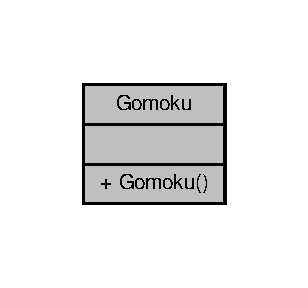
\includegraphics[width=148pt]{classGomoku__coll__graph}
\end{center}
\end{figure}


\subsection{Detailed Description}
Program main loop 

Definition at line 11 of file Gomoku.\+h.



The documentation for this class was generated from the following files\+:\begin{DoxyCompactItemize}
\item 
headers/Gomoku.\+h\item 
classes/Gomoku.\+cpp\end{DoxyCompactItemize}

\hypertarget{classLogger}{}\section{Logger Class Reference}
\label{classLogger}\index{Logger@{Logger}}


{\ttfamily \#include $<$Logger.\+h$>$}



Collaboration diagram for Logger\+:
\nopagebreak
\begin{figure}[H]
\begin{center}
\leavevmode
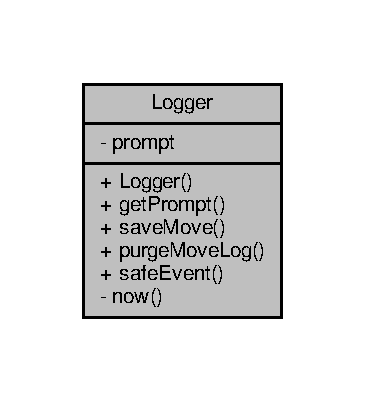
\includegraphics[width=175pt]{classLogger__coll__graph}
\end{center}
\end{figure}
\subsection*{Static Public Member Functions}
\begin{DoxyCompactItemize}
\item 
static std\+::string \hyperlink{classLogger_a4004f551a3c44ceb479c7c36e4e1dee8}{get\+Prompt} ()
\item 
static void \hyperlink{classLogger_a1e920507694b06e8a16120783902e229}{save\+Move} (int x, int y, char symbol)
\item 
static void \hyperlink{classLogger_a69ca833f3e3643333d718f0cce464f9b}{purge\+Move\+Log} ()
\item 
static void \hyperlink{classLogger_ad2156c976610010c579352c9aeb4b388}{safe\+Event} (std\+::string event)
\end{DoxyCompactItemize}
\subsection*{Static Private Member Functions}
\begin{DoxyCompactItemize}
\item 
static std\+::string \hyperlink{classLogger_a756a608050fea9f497dd2736f9321f3b}{now} ()
\end{DoxyCompactItemize}
\subsection*{Static Private Attributes}
\begin{DoxyCompactItemize}
\item 
static const std\+::string \hyperlink{classLogger_a80c00c4446e4310cfbf9ed048edbe979}{prompt} = \char`\"{}-\/-\/$>$\char`\"{}
\end{DoxyCompactItemize}


\subsection{Detailed Description}
Facility used to save vital information about processing states and events, for after release program care 

Definition at line 16 of file Logger.\+h.



\subsection{Member Function Documentation}
\mbox{\Hypertarget{classLogger_a4004f551a3c44ceb479c7c36e4e1dee8}\label{classLogger_a4004f551a3c44ceb479c7c36e4e1dee8}} 
\index{Logger@{Logger}!get\+Prompt@{get\+Prompt}}
\index{get\+Prompt@{get\+Prompt}!Logger@{Logger}}
\subsubsection{\texorpdfstring{get\+Prompt()}{getPrompt()}}
{\footnotesize\ttfamily std\+::string Logger\+::get\+Prompt (\begin{DoxyParamCaption}{ }\end{DoxyParamCaption})\hspace{0.3cm}{\ttfamily [static]}}

Returns setup propmpt symbol \begin{DoxyReturn}{Returns}

\end{DoxyReturn}


Definition at line 50 of file Logger.\+cpp.

\mbox{\Hypertarget{classLogger_a756a608050fea9f497dd2736f9321f3b}\label{classLogger_a756a608050fea9f497dd2736f9321f3b}} 
\index{Logger@{Logger}!now@{now}}
\index{now@{now}!Logger@{Logger}}
\subsubsection{\texorpdfstring{now()}{now()}}
{\footnotesize\ttfamily std\+::string Logger\+::now (\begin{DoxyParamCaption}{ }\end{DoxyParamCaption})\hspace{0.3cm}{\ttfamily [static]}, {\ttfamily [private]}}

Current date as U\+TM format \begin{DoxyReturn}{Returns}
string with date 
\end{DoxyReturn}


Definition at line 45 of file Logger.\+cpp.

\mbox{\Hypertarget{classLogger_a69ca833f3e3643333d718f0cce464f9b}\label{classLogger_a69ca833f3e3643333d718f0cce464f9b}} 
\index{Logger@{Logger}!purge\+Move\+Log@{purge\+Move\+Log}}
\index{purge\+Move\+Log@{purge\+Move\+Log}!Logger@{Logger}}
\subsubsection{\texorpdfstring{purge\+Move\+Log()}{purgeMoveLog()}}
{\footnotesize\ttfamily void Logger\+::purge\+Move\+Log (\begin{DoxyParamCaption}{ }\end{DoxyParamCaption})\hspace{0.3cm}{\ttfamily [static]}}

Used to purge mvoe log. Used in early versions, now useless \begin{DoxyRefDesc}{Deprecated}
\item[\hyperlink{deprecated__deprecated000001}{Deprecated}]\end{DoxyRefDesc}


Definition at line 30 of file Logger.\+cpp.

\mbox{\Hypertarget{classLogger_ad2156c976610010c579352c9aeb4b388}\label{classLogger_ad2156c976610010c579352c9aeb4b388}} 
\index{Logger@{Logger}!safe\+Event@{safe\+Event}}
\index{safe\+Event@{safe\+Event}!Logger@{Logger}}
\subsubsection{\texorpdfstring{safe\+Event()}{safeEvent()}}
{\footnotesize\ttfamily void Logger\+::safe\+Event (\begin{DoxyParamCaption}\item[{std\+::string}]{event }\end{DoxyParamCaption})\hspace{0.3cm}{\ttfamily [static]}}

Save all events in program to main log -\/$>$ log.\+log.\+log 
\begin{DoxyParams}{Parameters}
{\em event} & data to save \\
\hline
\end{DoxyParams}


Definition at line 37 of file Logger.\+cpp.

\mbox{\Hypertarget{classLogger_a1e920507694b06e8a16120783902e229}\label{classLogger_a1e920507694b06e8a16120783902e229}} 
\index{Logger@{Logger}!save\+Move@{save\+Move}}
\index{save\+Move@{save\+Move}!Logger@{Logger}}
\subsubsection{\texorpdfstring{save\+Move()}{saveMove()}}
{\footnotesize\ttfamily void Logger\+::save\+Move (\begin{DoxyParamCaption}\item[{int}]{x,  }\item[{int}]{y,  }\item[{char}]{symbol }\end{DoxyParamCaption})\hspace{0.3cm}{\ttfamily [static]}}

Save moves which made players to separate log -\/$>$ moves.\+log 
\begin{DoxyParams}{Parameters}
{\em x} & \\
\hline
{\em y} & \\
\hline
{\em symbol} & \\
\hline
\end{DoxyParams}


Definition at line 14 of file Logger.\+cpp.



\subsection{Member Data Documentation}
\mbox{\Hypertarget{classLogger_a80c00c4446e4310cfbf9ed048edbe979}\label{classLogger_a80c00c4446e4310cfbf9ed048edbe979}} 
\index{Logger@{Logger}!prompt@{prompt}}
\index{prompt@{prompt}!Logger@{Logger}}
\subsubsection{\texorpdfstring{prompt}{prompt}}
{\footnotesize\ttfamily const std\+::string Logger\+::prompt = \char`\"{}-\/-\/$>$\char`\"{}\hspace{0.3cm}{\ttfamily [static]}, {\ttfamily [private]}}

Prompt sign 

Definition at line 50 of file Logger.\+h.



The documentation for this class was generated from the following files\+:\begin{DoxyCompactItemize}
\item 
headers/Logger.\+h\item 
classes/Logger.\+cpp\end{DoxyCompactItemize}

\hypertarget{classMainMenu}{}\section{Main\+Menu Class Reference}
\label{classMainMenu}\index{Main\+Menu@{Main\+Menu}}


{\ttfamily \#include $<$Main\+Menu.\+h$>$}



Inheritance diagram for Main\+Menu\+:
\nopagebreak
\begin{figure}[H]
\begin{center}
\leavevmode
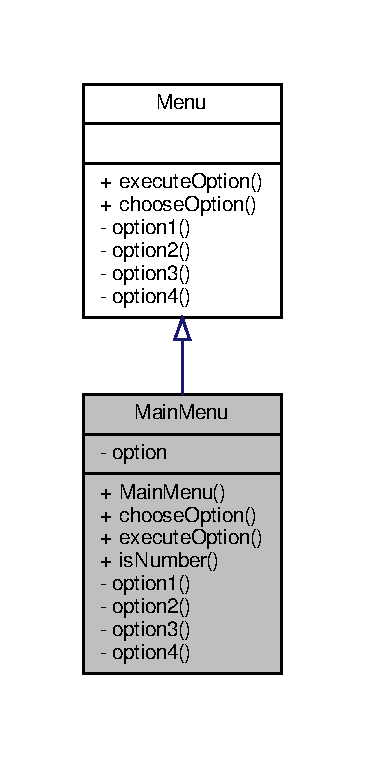
\includegraphics[width=175pt]{classMainMenu__inherit__graph}
\end{center}
\end{figure}


Collaboration diagram for Main\+Menu\+:
\nopagebreak
\begin{figure}[H]
\begin{center}
\leavevmode
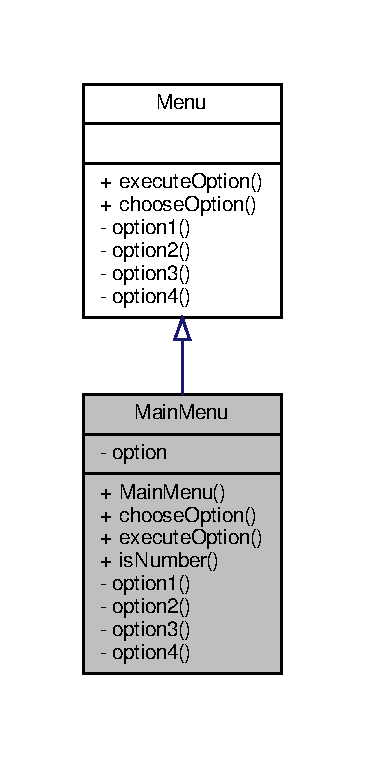
\includegraphics[width=175pt]{classMainMenu__coll__graph}
\end{center}
\end{figure}
\subsection*{Public Member Functions}
\begin{DoxyCompactItemize}
\item 
void \hyperlink{classMainMenu_a21c41131a13a5149fe5859d1d670e20b}{choose\+Option} () override
\item 
void \hyperlink{classMainMenu_adfc425f06cd51c10d78521315ae9abd6}{execute\+Option} () override
\item 
\mbox{\Hypertarget{classMainMenu_a8d9cc89fce7c6c8e1ec838d594add0b8}\label{classMainMenu_a8d9cc89fce7c6c8e1ec838d594add0b8}} 
void {\bfseries is\+Number} (std\+::string text)
\end{DoxyCompactItemize}
\subsection*{Private Member Functions}
\begin{DoxyCompactItemize}
\item 
void \hyperlink{classMainMenu_a783930d91ab415468d9c631eb61d0a00}{option1} () override
\item 
void \hyperlink{classMainMenu_a17f6460d8872b2ca269ebcf6eaa82589}{option2} () override
\item 
void \hyperlink{classMainMenu_a97fe096cec584b02614f759d7fcef8d1}{option3} () override
\item 
void \hyperlink{classMainMenu_a2097f6d1d30bad0b5c6e28575a48cc3e}{option4} () override
\end{DoxyCompactItemize}
\subsection*{Private Attributes}
\begin{DoxyCompactItemize}
\item 
\mbox{\Hypertarget{classMainMenu_a11e5e68dfcccc2b802d628043fd1694c}\label{classMainMenu_a11e5e68dfcccc2b802d628043fd1694c}} 
int {\bfseries option}
\end{DoxyCompactItemize}


\subsection{Detailed Description}
Main \hyperlink{classMenu}{Menu} class. Allows users to choose between\+: starting new game, continue last game, or see rankings 

Definition at line 16 of file Main\+Menu.\+h.



\subsection{Member Function Documentation}
\mbox{\Hypertarget{classMainMenu_a21c41131a13a5149fe5859d1d670e20b}\label{classMainMenu_a21c41131a13a5149fe5859d1d670e20b}} 
\index{Main\+Menu@{Main\+Menu}!choose\+Option@{choose\+Option}}
\index{choose\+Option@{choose\+Option}!Main\+Menu@{Main\+Menu}}
\subsubsection{\texorpdfstring{choose\+Option()}{chooseOption()}}
{\footnotesize\ttfamily void Main\+Menu\+::choose\+Option (\begin{DoxyParamCaption}{ }\end{DoxyParamCaption})\hspace{0.3cm}{\ttfamily [override]}, {\ttfamily [virtual]}}

Displays menu, and collects input 

Implements \hyperlink{classMenu}{Menu}.



Definition at line 34 of file Main\+Menu.\+cpp.

\mbox{\Hypertarget{classMainMenu_adfc425f06cd51c10d78521315ae9abd6}\label{classMainMenu_adfc425f06cd51c10d78521315ae9abd6}} 
\index{Main\+Menu@{Main\+Menu}!execute\+Option@{execute\+Option}}
\index{execute\+Option@{execute\+Option}!Main\+Menu@{Main\+Menu}}
\subsubsection{\texorpdfstring{execute\+Option()}{executeOption()}}
{\footnotesize\ttfamily void Main\+Menu\+::execute\+Option (\begin{DoxyParamCaption}{ }\end{DoxyParamCaption})\hspace{0.3cm}{\ttfamily [override]}, {\ttfamily [virtual]}}

Execute option chosen by user 

Implements \hyperlink{classMenu}{Menu}.



Definition at line 67 of file Main\+Menu.\+cpp.

\mbox{\Hypertarget{classMainMenu_a783930d91ab415468d9c631eb61d0a00}\label{classMainMenu_a783930d91ab415468d9c631eb61d0a00}} 
\index{Main\+Menu@{Main\+Menu}!option1@{option1}}
\index{option1@{option1}!Main\+Menu@{Main\+Menu}}
\subsubsection{\texorpdfstring{option1()}{option1()}}
{\footnotesize\ttfamily void Main\+Menu\+::option1 (\begin{DoxyParamCaption}{ }\end{DoxyParamCaption})\hspace{0.3cm}{\ttfamily [override]}, {\ttfamily [private]}, {\ttfamily [virtual]}}

Here used as New Game option 

Implements \hyperlink{classMenu}{Menu}.



Definition at line 12 of file Main\+Menu.\+cpp.

\mbox{\Hypertarget{classMainMenu_a17f6460d8872b2ca269ebcf6eaa82589}\label{classMainMenu_a17f6460d8872b2ca269ebcf6eaa82589}} 
\index{Main\+Menu@{Main\+Menu}!option2@{option2}}
\index{option2@{option2}!Main\+Menu@{Main\+Menu}}
\subsubsection{\texorpdfstring{option2()}{option2()}}
{\footnotesize\ttfamily void Main\+Menu\+::option2 (\begin{DoxyParamCaption}{ }\end{DoxyParamCaption})\hspace{0.3cm}{\ttfamily [override]}, {\ttfamily [private]}, {\ttfamily [virtual]}}

Here used as Continue option 

Implements \hyperlink{classMenu}{Menu}.



Definition at line 18 of file Main\+Menu.\+cpp.

\mbox{\Hypertarget{classMainMenu_a97fe096cec584b02614f759d7fcef8d1}\label{classMainMenu_a97fe096cec584b02614f759d7fcef8d1}} 
\index{Main\+Menu@{Main\+Menu}!option3@{option3}}
\index{option3@{option3}!Main\+Menu@{Main\+Menu}}
\subsubsection{\texorpdfstring{option3()}{option3()}}
{\footnotesize\ttfamily void Main\+Menu\+::option3 (\begin{DoxyParamCaption}{ }\end{DoxyParamCaption})\hspace{0.3cm}{\ttfamily [override]}, {\ttfamily [private]}, {\ttfamily [virtual]}}

Here used as See \hyperlink{classRanking}{Ranking} option 

Implements \hyperlink{classMenu}{Menu}.



Definition at line 24 of file Main\+Menu.\+cpp.

\mbox{\Hypertarget{classMainMenu_a2097f6d1d30bad0b5c6e28575a48cc3e}\label{classMainMenu_a2097f6d1d30bad0b5c6e28575a48cc3e}} 
\index{Main\+Menu@{Main\+Menu}!option4@{option4}}
\index{option4@{option4}!Main\+Menu@{Main\+Menu}}
\subsubsection{\texorpdfstring{option4()}{option4()}}
{\footnotesize\ttfamily void Main\+Menu\+::option4 (\begin{DoxyParamCaption}{ }\end{DoxyParamCaption})\hspace{0.3cm}{\ttfamily [override]}, {\ttfamily [private]}, {\ttfamily [virtual]}}

Never used here 

Implements \hyperlink{classMenu}{Menu}.



Definition at line 30 of file Main\+Menu.\+cpp.



The documentation for this class was generated from the following files\+:\begin{DoxyCompactItemize}
\item 
headers/Main\+Menu.\+h\item 
classes/Main\+Menu.\+cpp\end{DoxyCompactItemize}

\hypertarget{classMenu}{}\section{Menu Class Reference}
\label{classMenu}\index{Menu@{Menu}}


{\ttfamily \#include $<$Menu.\+h$>$}



Inheritance diagram for Menu\+:
\nopagebreak
\begin{figure}[H]
\begin{center}
\leavevmode
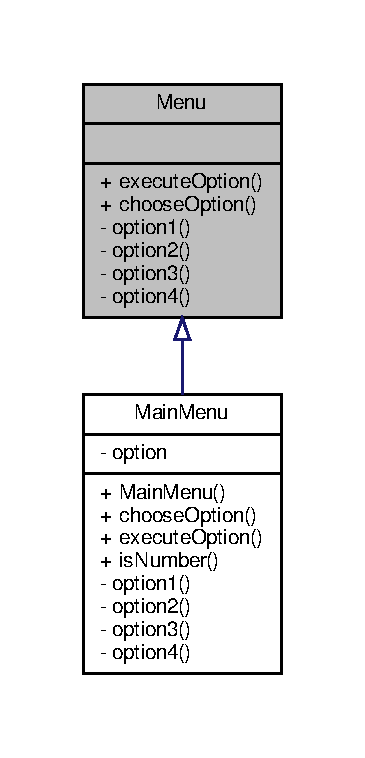
\includegraphics[width=175pt]{classMenu__inherit__graph}
\end{center}
\end{figure}


Collaboration diagram for Menu\+:
\nopagebreak
\begin{figure}[H]
\begin{center}
\leavevmode
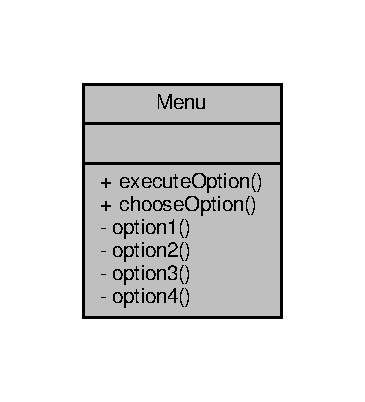
\includegraphics[width=175pt]{classMenu__coll__graph}
\end{center}
\end{figure}
\subsection*{Public Member Functions}
\begin{DoxyCompactItemize}
\item 
\mbox{\Hypertarget{classMenu_aa1725abe88c32d342bb81be3b7a58b3c}\label{classMenu_aa1725abe88c32d342bb81be3b7a58b3c}} 
virtual void {\bfseries execute\+Option} ()=0
\item 
\mbox{\Hypertarget{classMenu_acfdff87e19042816325dd4f99930843a}\label{classMenu_acfdff87e19042816325dd4f99930843a}} 
virtual void {\bfseries choose\+Option} ()=0
\end{DoxyCompactItemize}
\subsection*{Private Member Functions}
\begin{DoxyCompactItemize}
\item 
\mbox{\Hypertarget{classMenu_ad78c6112dae7a98bff166136fd52365a}\label{classMenu_ad78c6112dae7a98bff166136fd52365a}} 
virtual void {\bfseries option1} ()=0
\item 
\mbox{\Hypertarget{classMenu_a256af8b3454cd55d2f66e8db6d051e95}\label{classMenu_a256af8b3454cd55d2f66e8db6d051e95}} 
virtual void {\bfseries option2} ()=0
\item 
\mbox{\Hypertarget{classMenu_a68e18de4624af35fe1f339dfcb2f2813}\label{classMenu_a68e18de4624af35fe1f339dfcb2f2813}} 
virtual void {\bfseries option3} ()=0
\item 
\mbox{\Hypertarget{classMenu_a33fe544a273f2851280e3334ef728dac}\label{classMenu_a33fe544a273f2851280e3334ef728dac}} 
virtual void {\bfseries option4} ()=0
\end{DoxyCompactItemize}


\subsection{Detailed Description}
Abstract class for menu creation. Each menu can have up to 4 options. Process of collecting response, and executing it is separated into two different funcitons \begin{DoxySeeAlso}{See also}
\hyperlink{classMainMenu}{Main\+Menu} 
\end{DoxySeeAlso}


Definition at line 14 of file Menu.\+h.



The documentation for this class was generated from the following file\+:\begin{DoxyCompactItemize}
\item 
headers/Menu.\+h\end{DoxyCompactItemize}

\hypertarget{classRanking}{}\section{Ranking Class Reference}
\label{classRanking}\index{Ranking@{Ranking}}


{\ttfamily \#include $<$Ranking.\+h$>$}



Collaboration diagram for Ranking\+:
\nopagebreak
\begin{figure}[H]
\begin{center}
\leavevmode
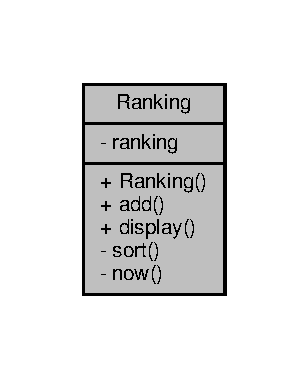
\includegraphics[width=148pt]{classRanking__coll__graph}
\end{center}
\end{figure}
\subsection*{Public Member Functions}
\begin{DoxyCompactItemize}
\item 
void \hyperlink{classRanking_a4969110ba50a492be5d125c9b1710cf0}{add} (int value)
\item 
void \hyperlink{classRanking_ade50abc368e58d4c7879e437f819e982}{display} (int amount)
\end{DoxyCompactItemize}
\subsection*{Private Member Functions}
\begin{DoxyCompactItemize}
\item 
void \hyperlink{classRanking_aa77c088257f2ac17f165147283136016}{sort} ()
\item 
std\+::string \hyperlink{classRanking_aa3ed270c7a8a059568c3af87fd73bd03}{now} ()
\end{DoxyCompactItemize}
\subsection*{Private Attributes}
\begin{DoxyCompactItemize}
\item 
std\+::vector$<$ std\+::pair$<$ int, std\+::string $>$ $>$ \hyperlink{classRanking_aead444bd691bbfa450ccdec64012ab86}{ranking}
\end{DoxyCompactItemize}


\subsection{Detailed Description}
Facility used to collect data about best results achieved by players. All data are saved to ranking.\+r file. Facility don\textquotesingle{}t have self contained list/vector of best result. Operation saving and reading results is operating on file each time. This approach saves R\+AM space, especially if there is a lots of data on record 

Definition at line 17 of file Ranking.\+h.



\subsection{Member Function Documentation}
\mbox{\Hypertarget{classRanking_a4969110ba50a492be5d125c9b1710cf0}\label{classRanking_a4969110ba50a492be5d125c9b1710cf0}} 
\index{Ranking@{Ranking}!add@{add}}
\index{add@{add}!Ranking@{Ranking}}
\subsubsection{\texorpdfstring{add()}{add()}}
{\footnotesize\ttfamily void Ranking\+::add (\begin{DoxyParamCaption}\item[{int}]{value }\end{DoxyParamCaption})}

Appends value to record.\+r file 
\begin{DoxyParams}{Parameters}
{\em value} & to append \\
\hline
\end{DoxyParams}


Definition at line 20 of file Ranking.\+cpp.

\mbox{\Hypertarget{classRanking_ade50abc368e58d4c7879e437f819e982}\label{classRanking_ade50abc368e58d4c7879e437f819e982}} 
\index{Ranking@{Ranking}!display@{display}}
\index{display@{display}!Ranking@{Ranking}}
\subsubsection{\texorpdfstring{display()}{display()}}
{\footnotesize\ttfamily void Ranking\+::display (\begin{DoxyParamCaption}\item[{int}]{amount }\end{DoxyParamCaption})}

Reads data from record.\+r file, sort it and display 
\begin{DoxyParams}{Parameters}
{\em amount} & of data to display \\
\hline
\end{DoxyParams}


Definition at line 27 of file Ranking.\+cpp.

\mbox{\Hypertarget{classRanking_aa3ed270c7a8a059568c3af87fd73bd03}\label{classRanking_aa3ed270c7a8a059568c3af87fd73bd03}} 
\index{Ranking@{Ranking}!now@{now}}
\index{now@{now}!Ranking@{Ranking}}
\subsubsection{\texorpdfstring{now()}{now()}}
{\footnotesize\ttfamily std\+::string Ranking\+::now (\begin{DoxyParamCaption}{ }\end{DoxyParamCaption})\hspace{0.3cm}{\ttfamily [private]}}

Current date as formated string \begin{DoxyReturn}{Returns}

\end{DoxyReturn}


Definition at line 49 of file Ranking.\+cpp.

\mbox{\Hypertarget{classRanking_aa77c088257f2ac17f165147283136016}\label{classRanking_aa77c088257f2ac17f165147283136016}} 
\index{Ranking@{Ranking}!sort@{sort}}
\index{sort@{sort}!Ranking@{Ranking}}
\subsubsection{\texorpdfstring{sort()}{sort()}}
{\footnotesize\ttfamily void Ranking\+::sort (\begin{DoxyParamCaption}{ }\end{DoxyParamCaption})\hspace{0.3cm}{\ttfamily [private]}}

Abstractions layer for std\+::sort 

Definition at line 12 of file Ranking.\+cpp.



\subsection{Member Data Documentation}
\mbox{\Hypertarget{classRanking_aead444bd691bbfa450ccdec64012ab86}\label{classRanking_aead444bd691bbfa450ccdec64012ab86}} 
\index{Ranking@{Ranking}!ranking@{ranking}}
\index{ranking@{ranking}!Ranking@{Ranking}}
\subsubsection{\texorpdfstring{ranking}{ranking}}
{\footnotesize\ttfamily std\+::vector$<$std\+::pair$<$int, std\+::string$>$ $>$ Ranking\+::ranking\hspace{0.3cm}{\ttfamily [private]}}

Vector with ranking, data are hold in it only for short while when user wants to see its records table. 

Definition at line 23 of file Ranking.\+h.



The documentation for this class was generated from the following files\+:\begin{DoxyCompactItemize}
\item 
headers/Ranking.\+h\item 
classes/Ranking.\+cpp\end{DoxyCompactItemize}

%--- End generated contents ---

% Index
\backmatter
\newpage
\phantomsection
\clearemptydoublepage
\addcontentsline{toc}{chapter}{Index}
\printindex

\end{document}
